All data provided by the challenge- and the "opendata.cern"-dataset \cite{higgsData} was created by the official ATLAS full detector simulator in a two-part-process. The simulator first reproduces proton-proton collisions, called \textit{events}. Then it tracks these via a virtual model of the ATLAS-detector, the resulting data emulates the statistical properties of the real events. By this procedure it is possible to exactly know if an event is a searched \textit{signal}, or \textit{background}. Signal-events are generated by tau tau decay of the Higgs Boson. Background-events originate from three known processes\footnote{decay of Z boson, W boson and a pair of top quarks \cite{higgsPaper}} which produce radiation similar to the signal \cite{higgsPaper}. The true \textit{class} of an event is contained in the feature \textit{Label} as "$s$" (signal) and "$b$" (background).

Every event has a feature \textit{Weight}, an artifact by the simulation. Summed, the weights are "an unbiased estimate of the expected number of events falling in the same region during a given fixed time interval. In our case, the weights correspond to the quantity of real data taken during the year 2012" \cite{higgsPaper}. This relation causes the weight-mean of signal-events to be considerably smaller than background-weights. We will see, that the challenges evaluation utilizes this to punish incorrectly classifying background as signal.

The features $Weight$ and $Label$ were originally only provided in the training-dataset. The data used in this thesis is expanded by complete $Weight$-, $Label$-features and the Kaggle-specific features $KaggleSet$ and $KaggleWeight$. Last one is a normalization of $Weight$ for the total number of signal- or background-events with the same $KaggleSet$ feature.
This information enables us recreating the challenges original datasets using the opendata.cern-dataset.

The physical features are separated in two types. Features containing so-called primitive data, properties of events explicitly measured by the simulated ATLAS detector, use the preamble "\textit{PRI\_}" in their names. The second type is called derived data, which are features that have been computed from primitive features. Their labels use the preamble "\textit{DER\_}".\\


\begin{table}[h]
	\begin{center}
		\begin{tabular}{ | c | c | c | c | c | c | c | }
		    \hline
		    EventID & DER\_mass\_MMC & \ldots & Weight & Label & KaggleSet & 
		    KaggleWeight \\
		    \hline
	    	133337  & 1.337   & \ldots & 0.4    & $s$ & $v$ & 0.04     \\
		    \hline
		\end{tabular} 
		\label{tab:data}
		\caption{Representation of the dataset}
	\end{center}
\end{table}


All features of the dataset are described more detailed in Appendix \ref{app:data}.

One might expect decent physics-knowledge as key in succeeding in the challenge, the top-participants did not use a lot domain-knowledge for feature- or method-selection. One goal of the challenges organization was to set a task for data scientists without any physics-background \cite{higgsPaper}.

\subsubsection{Data visualization}

In an first attempt to gain information about our data we use basic methods of data analysis.
To evaluate a training sets single feature for classification it is common to plot a histogram of the class-labels, in our case "$s$" and "$b$", distribution. A useful way to learn about relations between features is to create \textit{scatter plots} of all two-features-combinations.
Using these visualizations, we can identify features with good properties for our task.


%\begin{figure}[h]
%	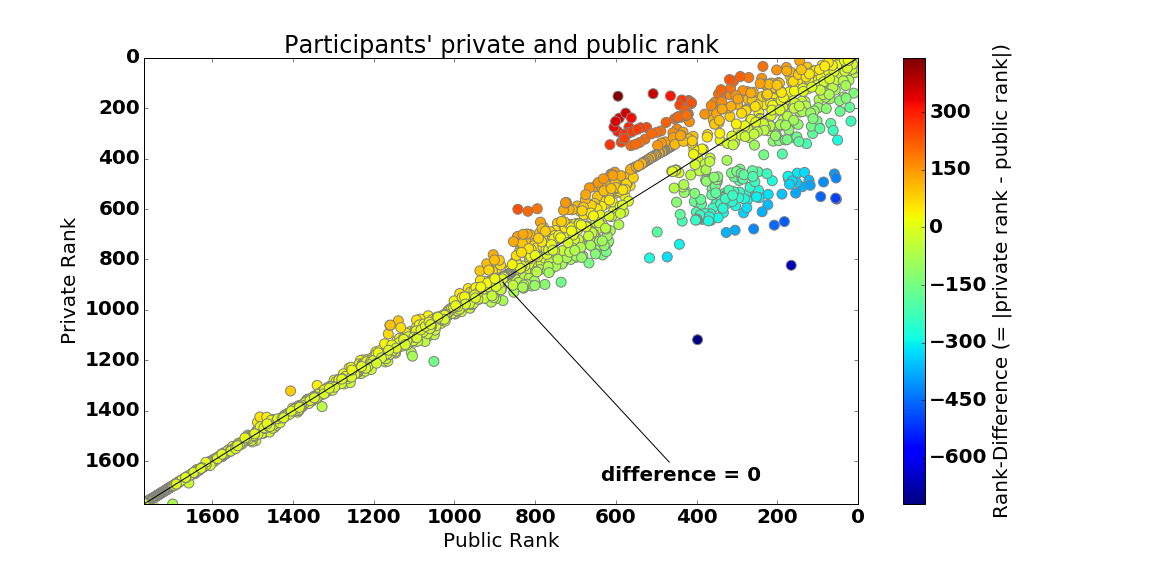
\includegraphics[width=0.5\textwidth]{images/privateVSpublic}
%	\caption{Put Histograms here!}
%\end{figure}
%\begin{figure}[h]
%	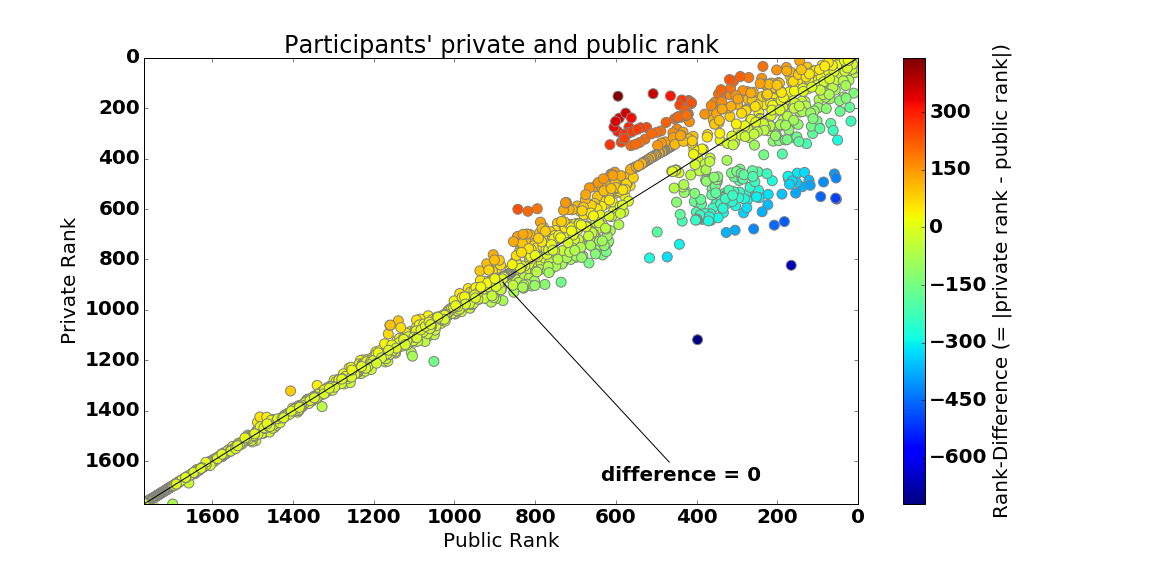
\includegraphics[width=0.5\textwidth]{images/privateVSpublic}
%	\caption{Put Scatter plots here!}
%\end{figure}

\begin{figure}[h]
\centering
\begin{minipage}{.5\textwidth}
  \centering
  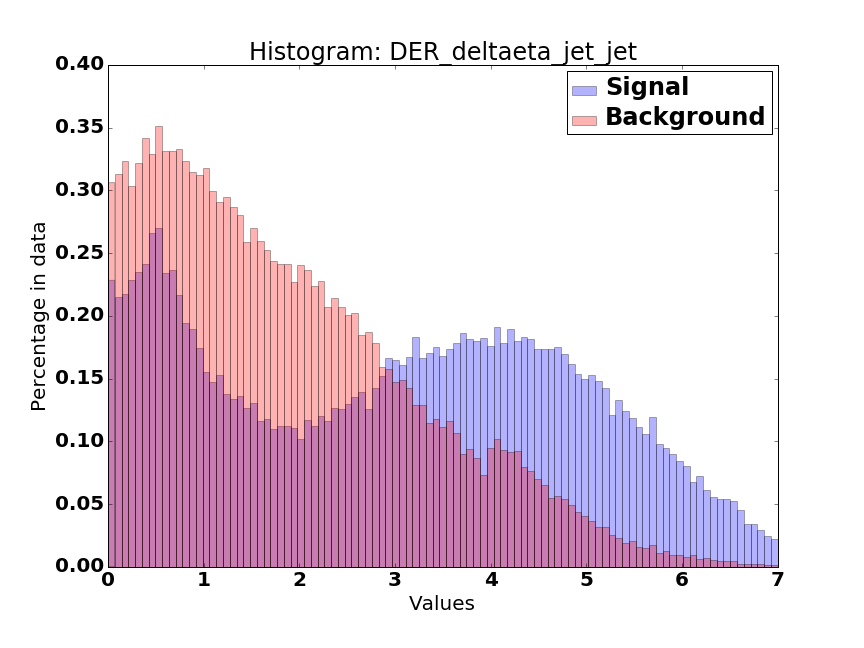
\includegraphics[width=\linewidth]{images/hist_DER_deltaeta_jet_jet}
  \captionof{figure}{\\ Histogram of \textit{DER\_deltaeta\_jet\_jet}}
  \label{fig:hist1}
\end{minipage}%
\begin{minipage}{.5\textwidth}
  \centering
  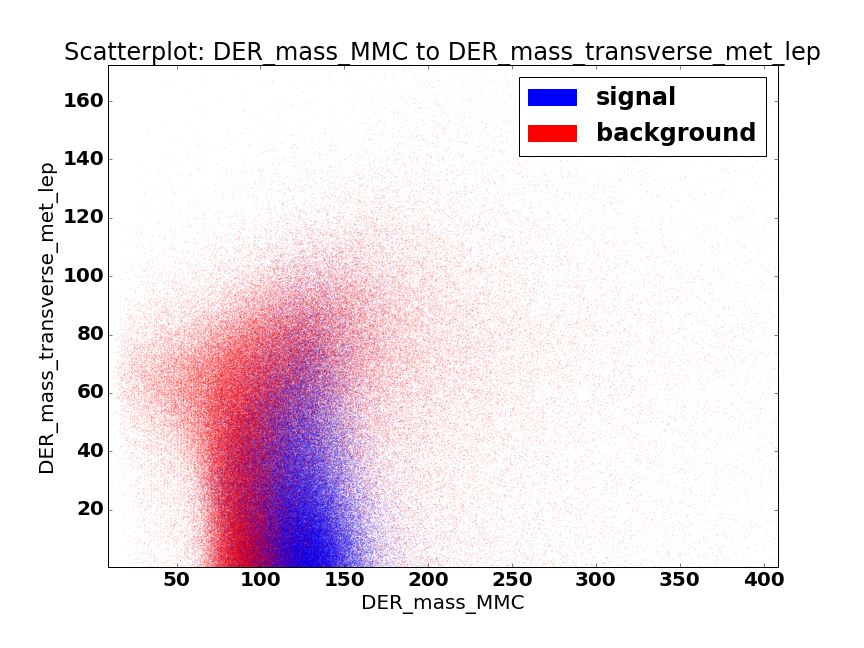
\includegraphics[width=\linewidth]{images/scat_DER_mass_MMCtoDER_mass_transverse_met_lep}
  \captionof{figure}{Scatter plot of \textit{DER\_mass\_MMC} to \textit{DER\_mass\_transverse\_met\_lep}}
  \label{fig:scat1}
\end{minipage}
\end{figure}

